\documentclass[12pt,a4paper]{report}

% ==================== PACKAGES ====================
\usepackage[utf8]{inputenc}
\usepackage[T1]{fontenc}
\usepackage[margin=0.85in, top=0.9in, bottom=0.9in]{geometry}
\usepackage{graphicx}
\usepackage{float}
\usepackage{xcolor}
\usepackage{listings}
\usepackage{array}
\usepackage{booktabs}
\usepackage{setspace}
\usepackage{fancyhdr}
\usepackage{titlesec}
\usepackage[hidelinks]{hyperref}
\usepackage{amsmath}
\usepackage{amssymb}

% ==================== PAGE STYLE ====================
\onehalfspacing
\setlength{\parindent}{0pt}
\setlength{\parskip}{6pt}

\pagestyle{fancy}
\fancyhf{}
\lhead{Computer Graphics Lab}
\rhead{Cyberpunk City Visualization}
\cfoot{\thepage}
\renewcommand{\headrulewidth}{0.4pt}

% ==================== CHAPTER STYLE ====================
\titleformat{\chapter}
{\normalfont\LARGE\bfseries}
{\thechapter.}
{10pt}
{}

\titlespacing*{\chapter}{0pt}{-10pt}{18pt}
\titlespacing*{\section}{0pt}{10pt}{5pt}

% ==================== COLORS ====================
\definecolor{codebg}{RGB}{248,248,248}

% ==================== CODE STYLE ====================
\lstset{
    language=C++,
    basicstyle=\ttfamily\small,
    keywordstyle=\color{blue}\bfseries,
    commentstyle=\color{gray},
    stringstyle=\color{red},
    backgroundcolor=\color{codebg},
    frame=single,
    breaklines=true,
    showstringspaces=false,
    tabsize=4,
    numbers=left,
    numberstyle=\tiny\color{gray}
}

\begin{document}

% ==================== TITLE PAGE ====================
\begin{titlepage}
    \centering
    \vspace*{1.8cm}

    {\Huge \textbf{Cyberpunk Neon Rainy City Visualization}}\\[0.5cm]
    {\Large A 3D Interactive Graphics Application using OpenGL and GLUT}\\[1.3cm]

    \rule{0.85\textwidth}{0.5pt}\\[0.8cm]

    {\Large \textbf{Lab Report}}\\[1.3cm]

    \begin{tabular}{rl}
        \textbf{Name:} & MD. Sujon Mahamud \\
        \textbf{Student ID:} & 223400039\\
        \textbf{Semester:} & Spring 2026 \\
        \textbf{Course Code:} & CSE 412 \\
        \textbf{Course Title:} & Computer Graphics Lab \\
        \textbf{Project Type:} & Mini Project \\
        \textbf{Language:} & C++ \\
        \textbf{Graphics Library:} & OpenGL and GLUT \\
        \textbf{Date:} & \today \\
    \end{tabular}

    \vfill
    \rule{0.85\textwidth}{0.5pt}\\[0.3cm]
    {\large Department of Computer Science and Engineering}
\end{titlepage}

\tableofcontents
\newpage

% ==================== ABSTRACT ====================
\chapter*{Abstract}
\addcontentsline{toc}{chapter}{Abstract}

This report presents an interactive 3D graphics project titled \textbf{Cyberpunk Neon Rainy City Visualization}. The project was developed using C++, OpenGL, and GLUT. It demonstrates important computer graphics concepts such as 3D modeling, lighting, material properties, animation, particle systems, fog effect, and camera control.

The environment contains neon buildings, moving cars, a flying drone, rain animation, fog atmosphere, day/night mode, and a real-time clock on a building. The project creates a futuristic cyberpunk-style city and provides interactive keyboard controls for user navigation.

\textbf{Keywords:} OpenGL, GLUT, Computer Graphics, 3D City, Cyberpunk, Rain Animation

\newpage

% ==================== OBJECTIVE ====================
\chapter{Objective}

The main objective of this project is to design and implement an interactive 3D cyberpunk city environment using OpenGL and GLUT.

The specific objectives are:

\begin{enumerate}
    \item To create a realistic 3D city environment using OpenGL primitives.
    \item To apply lighting, shading, and material properties.
    \item To implement animated rain using a particle system.
    \item To add moving cars and a flying drone.
    \item To create day and night mode switching.
    \item To implement fog for atmospheric depth.
    \item To provide keyboard-based interactive camera controls.
\end{enumerate}

% ==================== INTRODUCTION ====================
\chapter{Introduction}

Computer Graphics is an important field of computer science that deals with creating and manipulating visual content using computers. OpenGL is a widely used graphics library for developing 2D and 3D applications.

In this project, a futuristic cyberpunk city was created using OpenGL and GLUT. The scene is inspired by modern cyberpunk environments where neon lights, dark roads, rain, fog, and tall buildings create a futuristic atmosphere.

The project includes several interactive and animated elements such as moving cars, animated rain, flying drone, day/night switching, and a real-time building clock.

% ==================== DESIGN DETAILS ====================
\chapter{Design Details}

\section{Scene Components}

The scene is divided into several components. Each component is created using OpenGL primitives and transformations.

\begin{table}[H]
\centering
\renewcommand{\arraystretch}{1.3}
\begin{tabular}{|p{4cm}|p{9cm}|}
\hline
\textbf{Component} & \textbf{Description} \\
\hline
Buildings & Multiple cyberpunk-style buildings with neon windows. \\
\hline
Road & A central road with lane markings and neon side lights. \\
\hline
Sidewalks & Walkways placed on both sides of the road. \\
\hline
Cars & Three animated cars moving along the road. \\
\hline
Drone & A flying drone moving in circular motion. \\
\hline
Rain & Particle-based rain system using 650 particles. \\
\hline
Fog & Atmospheric fog effect for depth and realism. \\
\hline
Clock & A real-time analog clock placed on a building. \\
\hline
\end{tabular}
\caption{Main Components of the Project}
\end{table}

\section{Scene Structure}

\begin{figure}[H]
\centering
\begin{verbatim}
Scene Root
|-- Sky
|-- Ground
|-- Road
|-- Sidewalks
|-- Buildings
|-- Cars
|-- Drone
|-- Street Lights
|-- Billboards
|-- Rain Particles
|-- Clock Building
\end{verbatim}
\caption{Scene Hierarchy}
\end{figure}

\section{Lighting Design}

The project includes two lighting modes:

\begin{itemize}
    \item \textbf{Day Mode:} Bright sky, sunlight, and clear visibility.
    \item \textbf{Night Mode:} Dark background, moonlight, neon cyan and magenta lights.
\end{itemize}

Night mode creates the main cyberpunk effect using glowing neon colors and fog.

\begin{figure}[H]
\centering
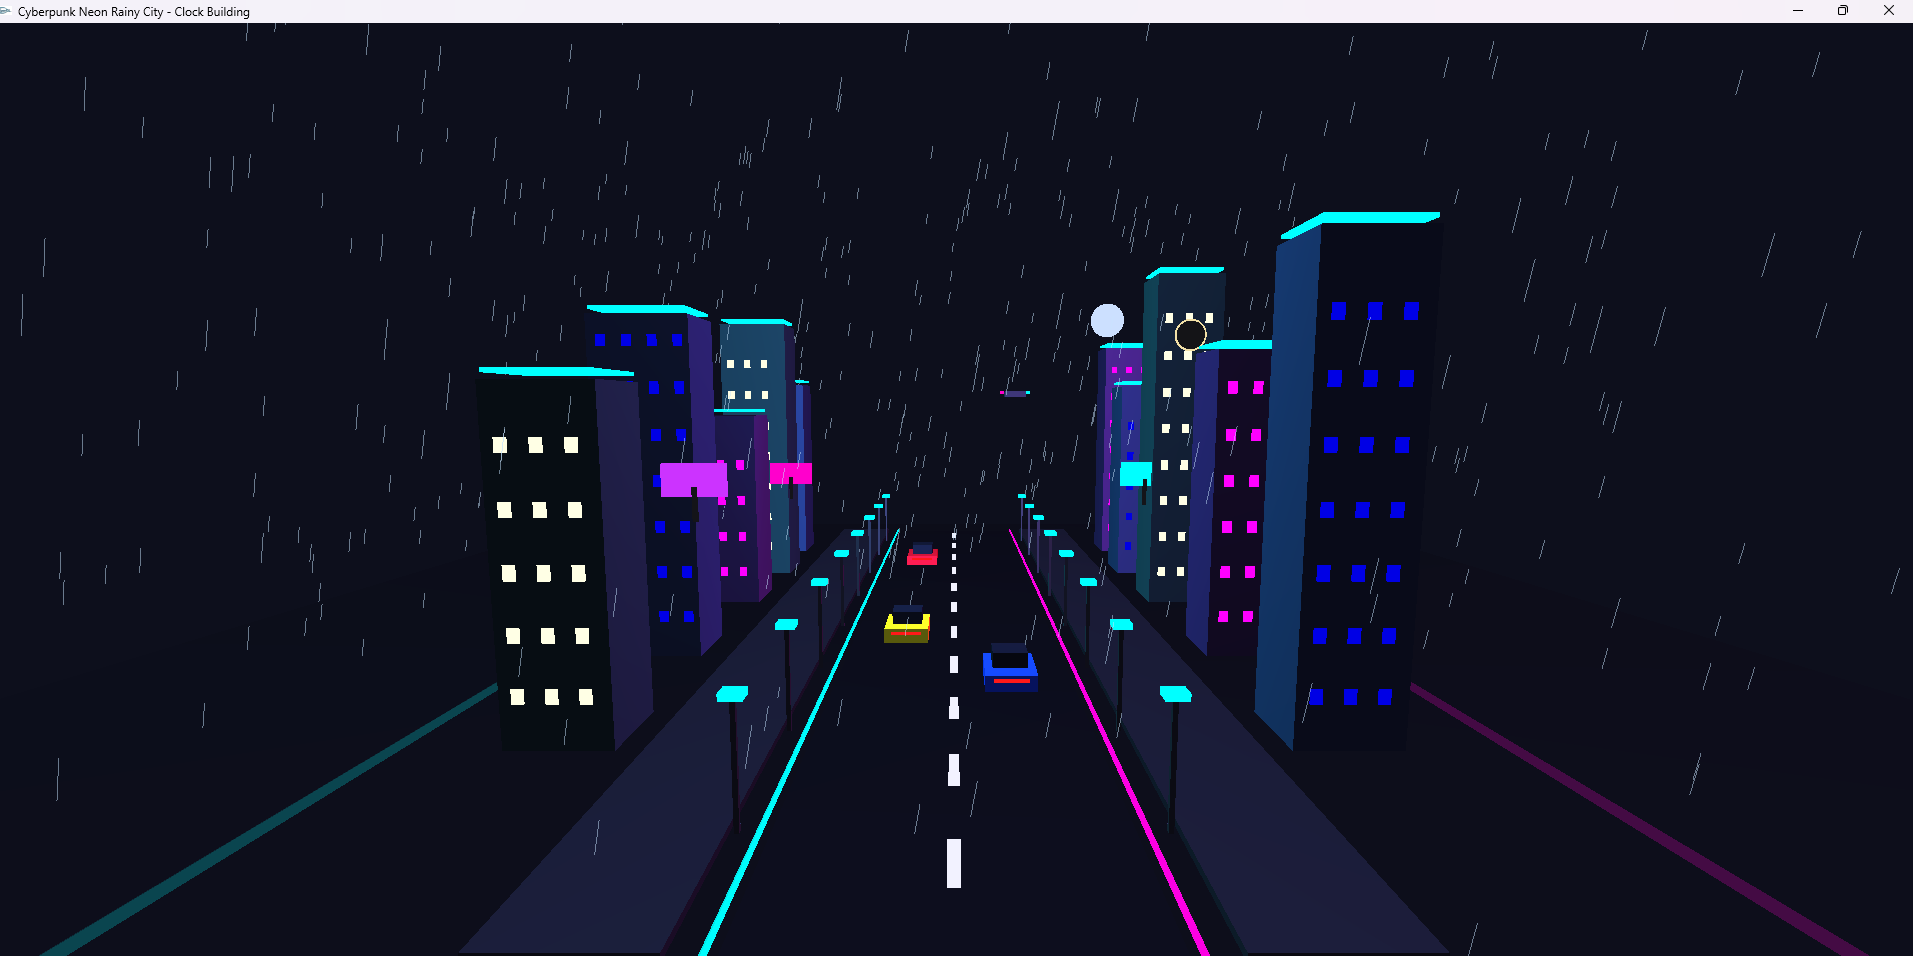
\includegraphics[width=0.92\textwidth]{fogandrain.png}
\caption{Cyberpunk Night Mode with Rain and Fog Effect}
\label{fig:lightingfog}
\end{figure}

% ==================== TECHNICAL IMPLEMENTATION ====================
\chapter{Technical Implementation}

\section{Libraries Used}

The following libraries were used in the project:

\begin{lstlisting}
#include <windows.h>
#include <GL/glut.h>
#include <cmath>
#include <cstdlib>
#include <ctime>
\end{lstlisting}

\section{Material Function}

A material function was used to control color, reflection, and shininess of objects.

\begin{lstlisting}
void setMaterial(float r, float g, float b, float shine) {
    GLfloat ambient[]  = { r * 0.45f, g * 0.45f, b * 0.45f, 1.0f };
    GLfloat diffuse[]  = { r, g, b, 1.0f };
    GLfloat specular[] = { 0.85f, 0.85f, 0.85f, 1.0f };

    glMaterialfv(GL_FRONT, GL_AMBIENT, ambient);
    glMaterialfv(GL_FRONT, GL_DIFFUSE, diffuse);
    glMaterialfv(GL_FRONT, GL_SPECULAR, specular);
    glMaterialf(GL_FRONT, GL_SHININESS, shine);
}
\end{lstlisting}

\section{Rain Particle System}

The rain system was implemented using a structure.

\begin{lstlisting}
struct Rain {
    float x, y, z;
    float speed;
};
\end{lstlisting}

Each raindrop has its own position and falling speed. The rain particles are updated continuously to create an animated rainfall effect.

\section{Camera Control}

The camera was implemented using \texttt{gluLookAt()}.

\begin{lstlisting}
gluLookAt(camX, camY, camZ,
          0, 2.5f, 0,
          0, 1, 0);
\end{lstlisting}

This allows the user to view the 3D scene from different positions.

\section{Animation}

Animation was implemented using the GLUT timer function.

\begin{lstlisting}
glutTimerFunc(16, update, 0);
\end{lstlisting}

This updates the scene approximately 60 times per second.

\section{Keyboard Controls}

\begin{table}[H]
\centering
\renewcommand{\arraystretch}{1.3}
\begin{tabular}{|c|p{8cm}|}
\hline
\textbf{Key} & \textbf{Function} \\
\hline
W / S & Zoom in and zoom out \\
\hline
A / D & Rotate the scene left and right \\
\hline
Q / E & Move camera up and down \\
\hline
Arrow Keys & Move camera position \\
\hline
R & Turn rain on or off \\
\hline
N & Turn neon lights on or off \\
\hline
T & Switch between day and night mode \\
\hline
F & Turn fog on or off \\
\hline
ESC & Exit the program \\
\hline
\end{tabular}
\caption{Keyboard Controls}
\end{table}

% ==================== DISCUSSION ====================
\chapter{Discussion}

This project demonstrates several important concepts of computer graphics. The use of lighting and material properties makes the objects look more realistic. The rain particle system adds environmental animation, while the moving cars and drone make the city feel dynamic.

The day/night switching system helps compare two different lighting environments. The fog effect improves the depth of the scene and creates a cinematic cyberpunk atmosphere.

\section{Achievements}

\begin{itemize}
    \item Created a complete 3D city environment.
    \item Added realistic neon lighting.
    \item Implemented animated rain.
    \item Added moving cars and drone.
    \item Added interactive keyboard controls.
    \item Implemented day/night mode and fog effect.
\end{itemize}

\section{Limitations}

\begin{itemize}
    \item Texture mapping was not used.
    \item No advanced shadow effect was implemented.
    \item Rain particles do not collide with buildings.
    \item No sound effect was added.
\end{itemize}

\section{Future Improvements}

\begin{itemize}
    \item Add texture mapping for buildings and roads.
    \item Add realistic shadows and reflections.
    \item Add sound effects for rain and traffic.
    \item Add first-person walking camera.
    \item Add more buildings and city objects.
\end{itemize}

% ==================== OUTPUT ====================
\chapter{Output}

The following screenshots show the final output of the Cyberpunk Neon Rainy City project.

\section{Output Screenshots}

\begin{figure}[H]
\centering
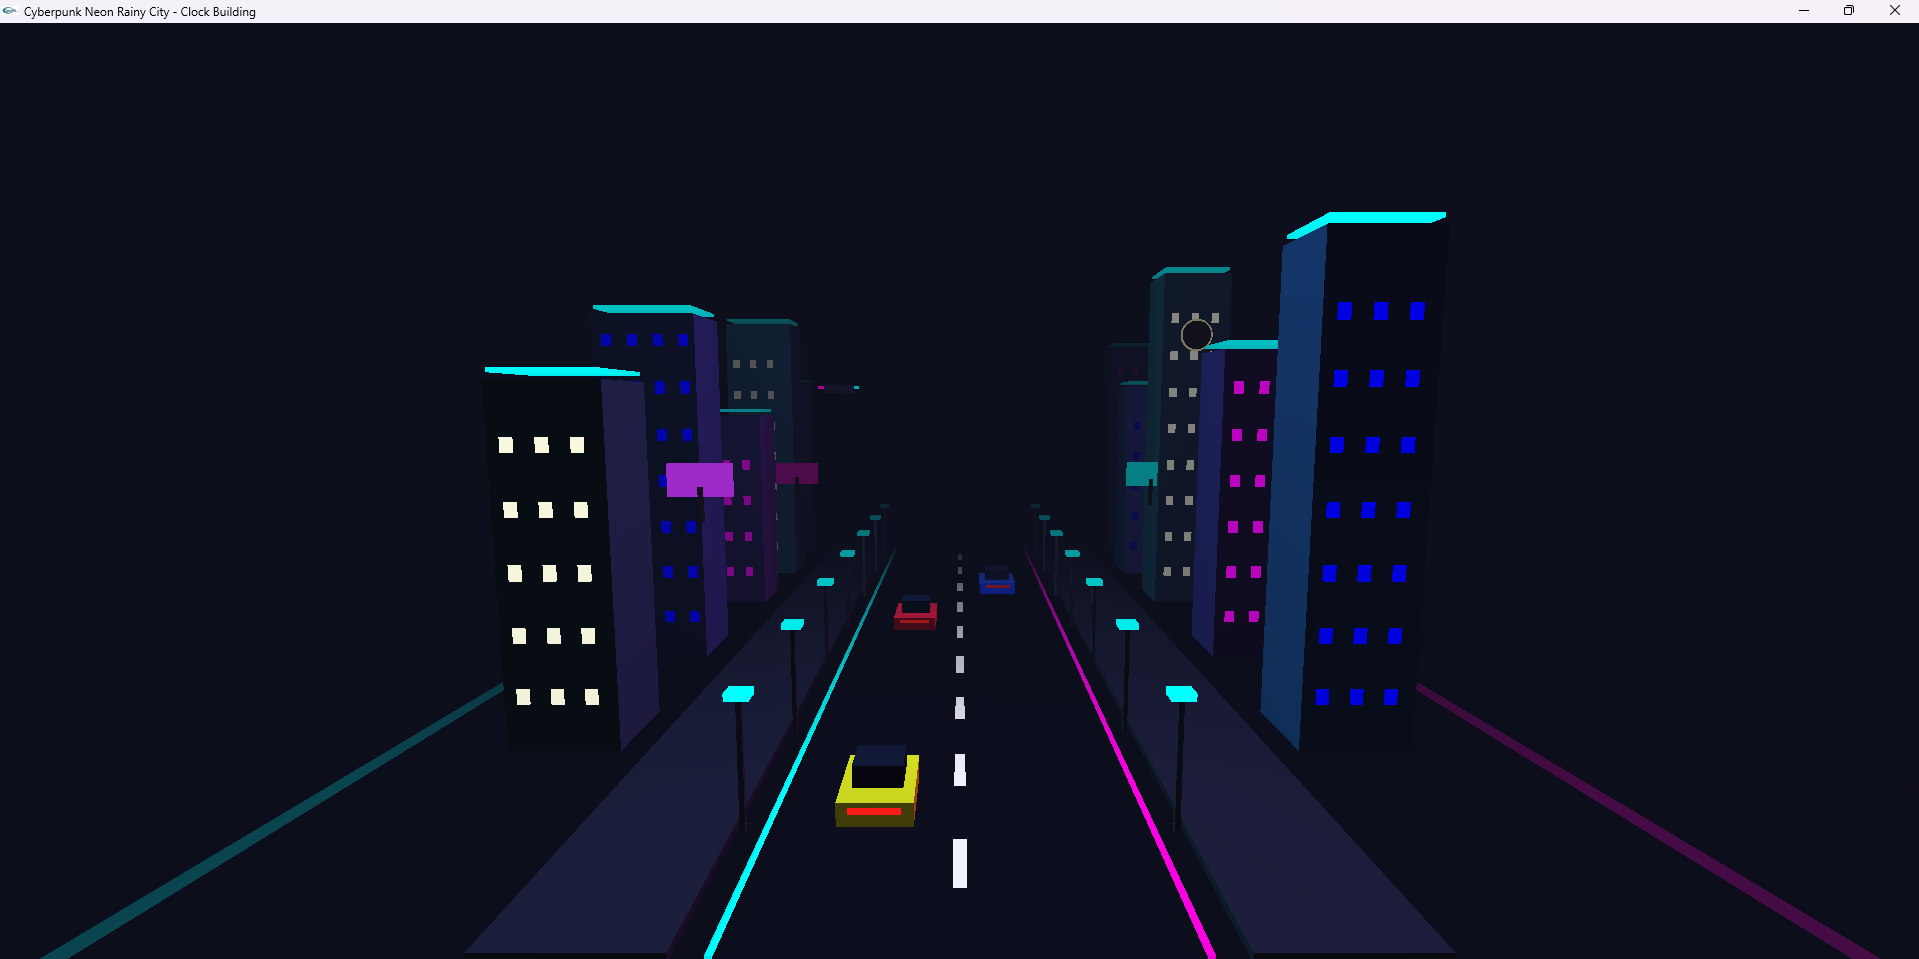
\includegraphics[width=0.92\textwidth]{nightmode.png}
\caption{Cyberpunk City in Night Mode}
\label{fig:nightmode}
\end{figure}

\begin{figure}[H]
\centering
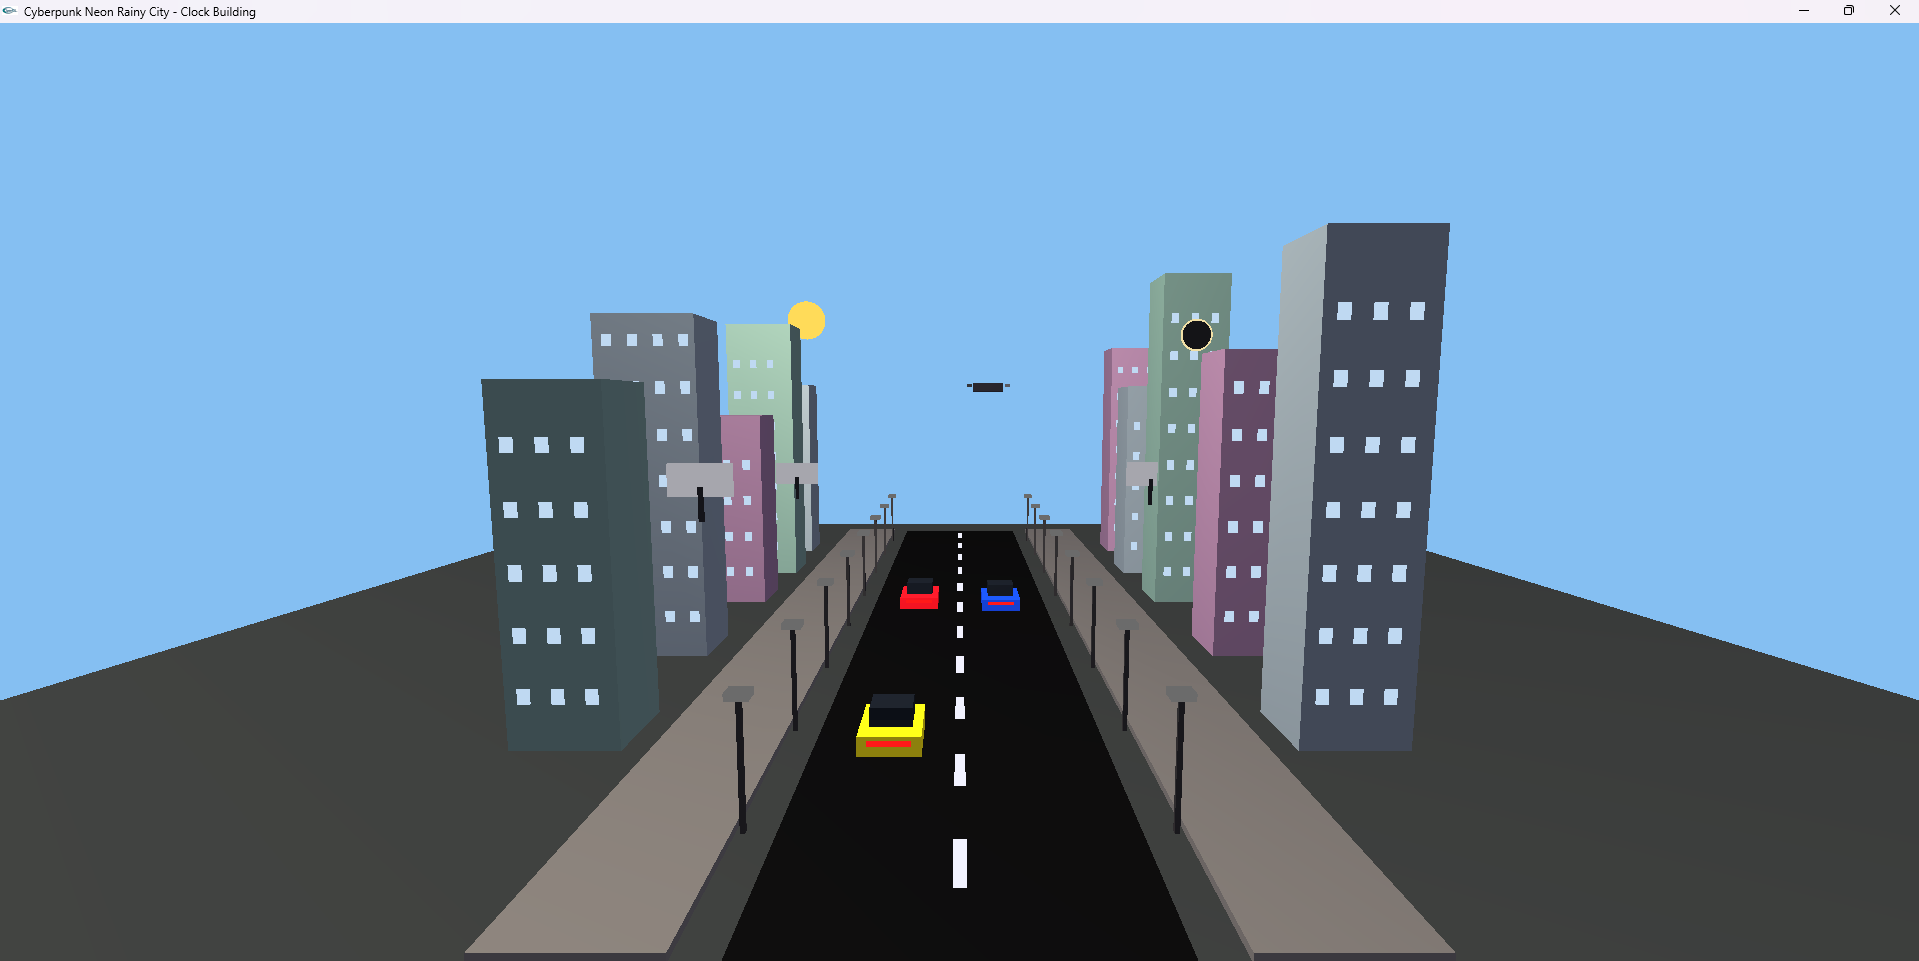
\includegraphics[width=0.92\textwidth]{daymode.png}
\caption{Cyberpunk City in Day Mode}
\label{fig:daymode}
\end{figure}

\begin{figure}[H]
\centering
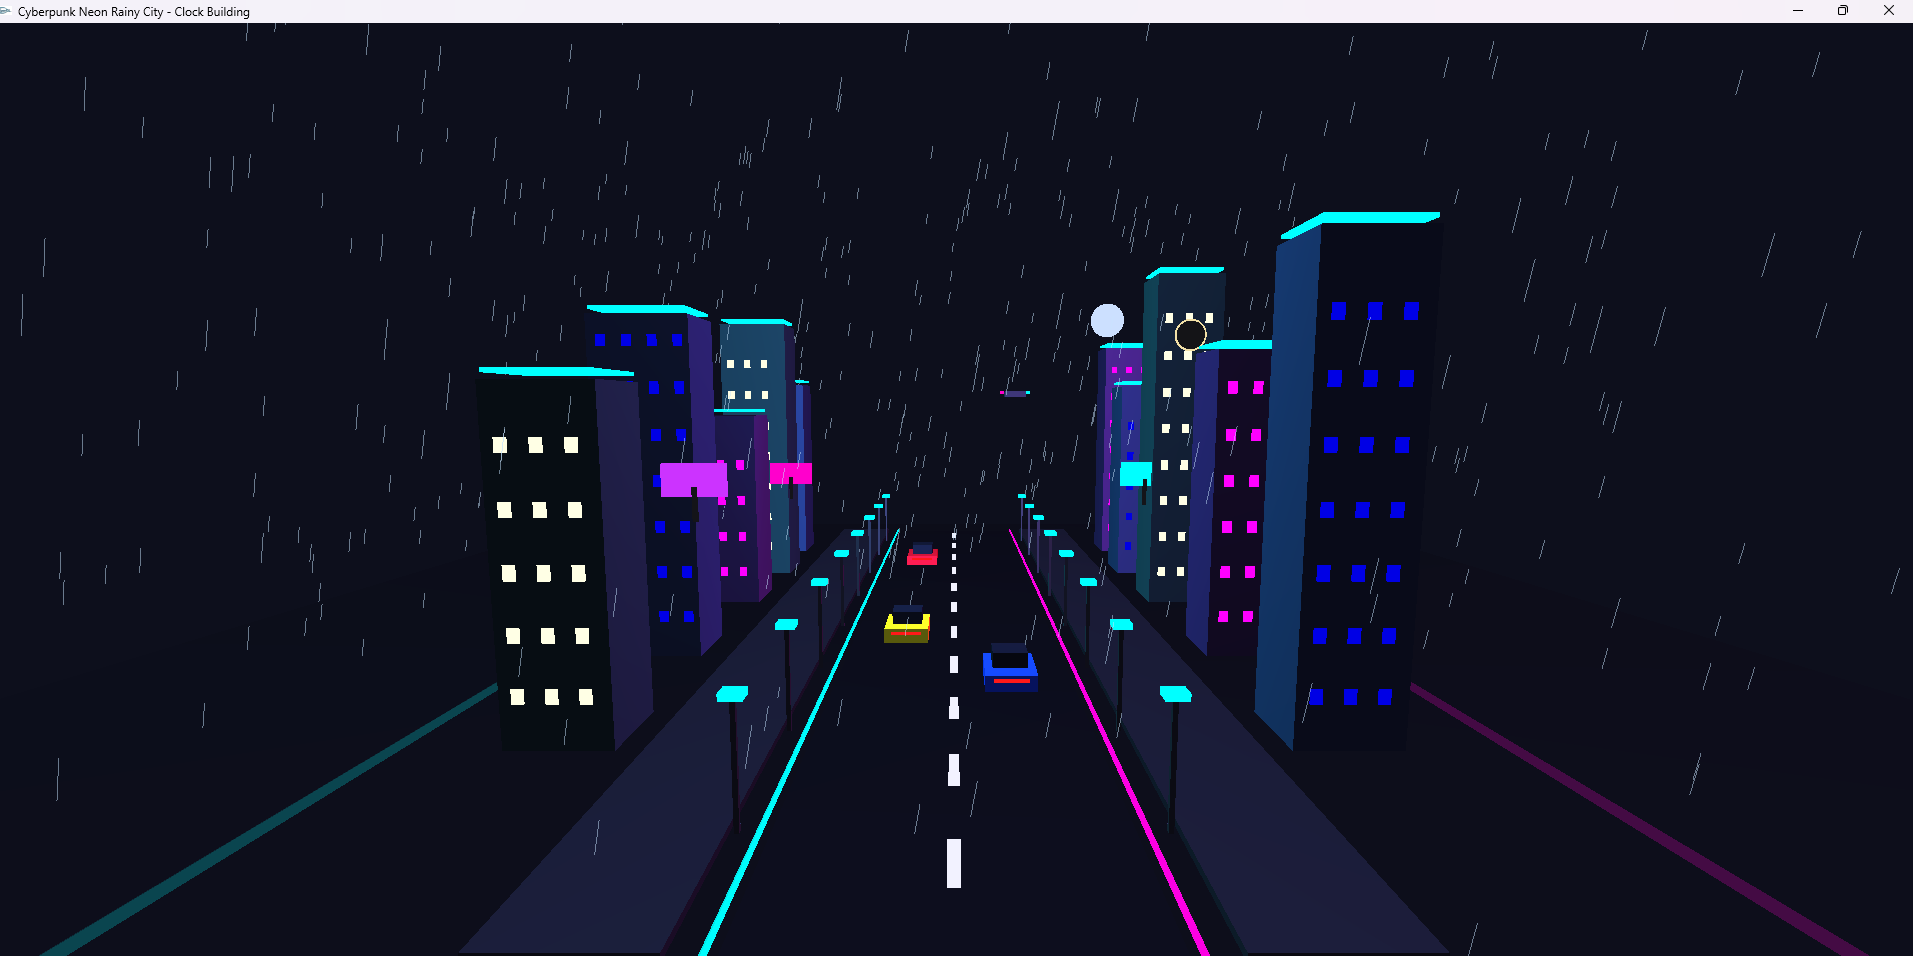
\includegraphics[width=0.92\textwidth]{fogandrain.png}
\caption{Cyberpunk City with Rain and Fog Effect}
\label{fig:fogandrain}
\end{figure}

% ==================== CONCLUSION ====================
\chapter{Conclusion}

The Cyberpunk Neon Rainy City project was successfully developed using OpenGL and GLUT. It demonstrates the practical use of 3D rendering, lighting, animation, fog, particle systems, and camera control.

The project achieved its main goal of creating an interactive and visually attractive cyberpunk city environment. It helped improve practical understanding of OpenGL programming and computer graphics concepts.

Overall, the project was completed successfully and fulfilled the expected objectives.

% ==================== REFERENCES ====================
\chapter{References}

\begin{enumerate}
    \item OpenGL Programming Guide.
    \item GLUT Documentation.
    \item Computer Graphics: Principles and Practice.
    \item Real-Time Rendering by Tomas Akenine-Möller.
\end{enumerate}

\end{document}
